\documentclass[a4paper,12pt]{article}

\usepackage{lab_preamble}

\begin{document}

\LabTitle{1.3.1 (первая часть) и 1.3.2 (вторая часть)}{Определение модуля Юнга по измерениям растяжения проволоки и Определение модуля сдвига при помощи крутильных колебаний}

\tableofcontents

\section{Первая часть.}

\paragraph{Цель работы}:
\begin{enumerate}
  \item экспериментально получить зависимость между напряжением и деформацией (закон Гука) для проволки
  \item по результатам измерений вычислить модуль Юнга
\end{enumerate}

\paragraph{Приборы}:
\begin{enumerate}
  \item прибор Лермантова
  \item проволока из исследуемого материала
  \item зрительная труба со шкалой
  \item набор грузов
  \item огромная линейка
\end{enumerate}

\subsection{Краткая Теория.}

\begin{figure} [h] \center
  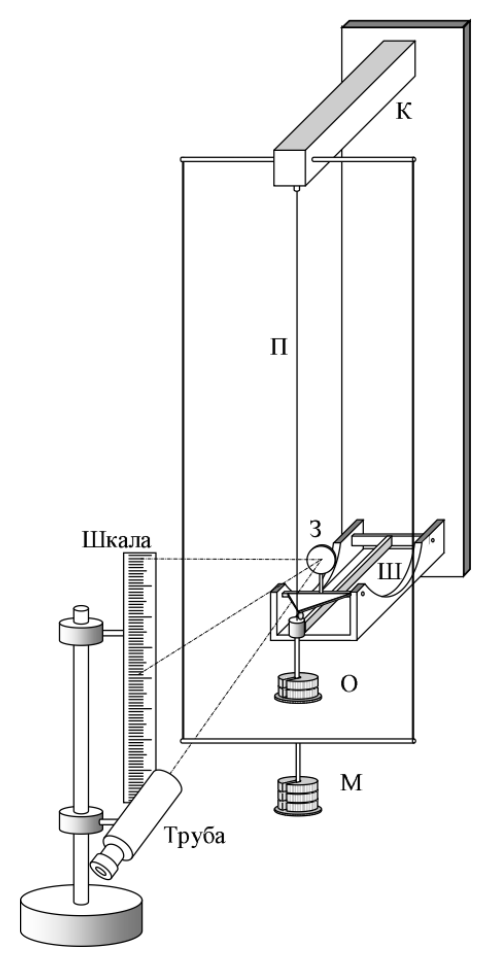
\includegraphics[scale=0.5]{131-132/pic 1.png}
  \caption[Рис. 1]{Прибор Лермантова} \label{pic:1}
\end{figure}

Для определения модуля Юнга проволки используется прибор Лермантова, схема которого изображена на рис. (\ref{pic:1}). Верхний конец проволоки П, изготовленной из исследуемого материала, прикреплен к консоли К, а нижний - к цилиндру, которым оканчивается шарнирный кронштейн Ш. На этот же цилиндр опирается рычаг r, связанный с зеркальцем З. Таким образом, удлинение проволоки можно измерить по углу по-ворота зеркальца.

Натяжение проволоки можно менять, перекладывая грузы с площадки М на площадку О и наоборот. Такая система позволяет исключить влияние деформации кронштейна К на точность измерений, так как нагрузка на нем все время остается постоянной.

Важно учитывать, что проволка всегда несколько изогнута.

Найти зависимость удлинения проволки $\D{\ell}$ от отклонения значения на линейке n можно найти по формуле:
\begin{equation}
  \D{l} = \frac{\D{x} \cdot r}{h} = \frac{r \cdot n \cdot (\cm)}{h}
  \label{eq:1.1}
\end{equation}

Закон Гука:
\begin{equation}
  P = E \cdot \frac{\D{\ell}}{l_0}
  \label{eq:1.2}
\end{equation}
где E - модуль юнга.

\subsection{Выполнение}
\begin{enumerate}
  \item \label{1:1} Диаметр проволки (d) должен быть написан на установке, если это не так, обратитесь к лектору. По диаметру найдем площадь поперечного сечения проволоки.

\[ d = (0,730 \pm 0,005) \text{мм} \]
\[ S = (0,420 \pm 0,006) \text{мм}^2 \] %!

  \item \label{1:2} Измерим длину проволоки.
  
\[ l_0 = (175,7 \pm 0,1) \text{см} \]

  \item \label{1:3} Направим зрительную трубу на зеркальце 3. Выведем формулу, связывающую число делений n по шкале, расстояние h от шкалы до зеркальца, длину рычага r и удлинение проволоки $\D{l}$. r указана на приборе, а расстояние h следует измерить огромной линейкой.

\[ r = (13 \pm 0) \text{мм} \]
\[ h = (144,1 \pm 0,1) \text{см} \]

Выведенная формула: \eqref{eq:1.1}

% таблица 1
\begin{table} [h] \center
\begin{tabular}{llll}
&значение&$\sigma$&$\eps$\\
\hline
d, мм&0.730&0.005&0.7\%\\
S, $\mm^2$&0.42&0.01&1.4\%\\
$\ell_0$, см&175.7&0.1&0.1\%\\
r, $\mm^2$&13.0&0.1&0.8\%\\
h, см&144.1&0.1&0.1\%\\
E, $\H/\mm^2$&91728&615&0.67\%\\
k, $\H/\mm$&21,9&0,3&1.53\%\\
масса, г&&0.1&\\
время, с&&0.6&\\
\end{tabular}
\caption{Значения \label{table:1}}
\end{table}

  \item \label{1:4} 

  Необходимо позаботиться о том, чтобы в процессе эксперимента не выйти за пределы области, где удлинение проволоки пропорционально ее натяжению (область пропорциональности). Оценим максимальную величину нагрузки, приняв, что разрушающее напряжение равно 900 Н/$\text{мм}^2$. Рабочее напряжение не должно превышать 30\% от величины разрушающего.

  Проверьте правильность сделанной оценки. Для этого нагрузите проволоку одним из имеющихся грузов, затем уберите его и посмотрите, вернулась ли длина проволоки к первоначальному значению. Повторите этот эксперимент с двумя, тремя и т. д. грузами, постепенно доходя до расчетной нагрузки. Если остаточные деформации станут заметными, дальнейшее увеличение нагрузки следует прекратить. При изменении нагрузки на проволоке каждый раз необходимо предварительно арретировать прибор (на рис. 1 арретир не показан).

  \item \label{1:5}  Снимим зависимость удлинения проволоки, то есть числа делений n по шкале, от массы грузов m при увеличении и уменьшении нагрузки. Повторите этот эксперимент 2-3 раза. (См. таблицу \ref{table:2} и \ref{table:3}) В таблице (\ref{table:2}): m - общая масса грузов, подвешенных на нить, $n_i$ - измеренное отклонение на шкале в см.
  
% таблица 2
\begin{table} [h] \center
\begin{tabular}{l|l|llll|l|lll|l}
  &m, г&$n_1$, см&$n_2$, см&$n_3$, см&$n_4$, см&$\avrg{n}$, см&$\sigma^{\text{случ}}_{\avrg{n}}$, см&$\sigma^{\text{приб}}_{\avrg{n}}$, см&$\sigma_{\avrg{n}}$, см&$\eps_{\avrg{n}}$\\
  \hline
  1&246&1.5&1.7&1.8&2&1.75&0.21&0.05&0.21&12\%\\
  2&491&2.8&3&3.2&3.4&3.1&0.26&0.05&0.26&8\%\\
  3&736&4.1&4.1&4.5&4.6&4.325&0.26&0.05&0.27&6\%\\
  4&982&5.2&5.4&5.8&5.7&5.525&0.28&0.05&0.28&5\%\\
  5&1228&6.4&6.6&7&7&6.75&0.30&0.05&0.30&5\%\\
  6&1474&7.7&7.8&8.5&8.2&8.05&0.37&0.05&0.37&5\%\\
  7&1719&8.9&9&9.5&9.5&9.225&0.32&0.05&0.32&4\%\\
  8&1965&10.2&10.3&10.8&10.7&10.5&0.29&0.05&0.30&3\%\\
  9&2211&11.1&11.5&12.1&12&11.675&0.46&0.05&0.47&4\%\\
  10&2457&12.2&12.2&13.2&13.2&12.7&0.58&0.05&0.58&5\%\\
\end{tabular}
\caption{Измерения \label{table:2}}
\begin{description}
  \item[m] - масса, подвешенная на проволоке
  \item[$n_i$] - отклонение от начального значения на шкале линейки
\end{description}
\end{table}

\begin{table} [h] \center
\begin{tabular}{l|lll|lll}
&P, $\frac{\H}{\mm^2}$&$\sigma_P$, $\frac{\H}{\mm^2}$&$\eps_P$&$\D{\ell}$, мм&$\sigma_{\D{\ell}}$, мм&$\eps_{\D{\ell}}$\\
\hline
1&5.8&0.1&1.4\%&0.158&0.019&12.3\%\\
2&11.5&0.2&1.4\%&0.280&0.024&8.5\%\\
3&17.3&0.2&1.4\%&0.390&0.024&6.2\%\\
4&23.0&0.3&1.4\%&0.498&0.026&5.1\%\\
5&28.8&0.4&1.4\%&0.609&0.028&4.6\%\\
6&34.6&0.5&1.4\%&0.726&0.034&4.7\%\\
7&40.3&0.6&1.4\%&0.832&0.030&3.6\%\\
8&46.1&0.6&1.4\%&0.947&0.028&2.9\%\\
9&51.8&0.7&1.4\%&1.053&0.043&4.1\%\\
10&57.6&0.8&1.4\%&1.146&0.053&4.6\%\\
\end{tabular}
\caption{P и $\D{l}$ \label{table:3}}
\end{table}

  \item \label{1:6} Построим график зависимости удлинения проволоки $\D{l}$ от нагрузки P. (См. рис. \ref{pic:2})
Должна получиться прямая. По ее наклону можно найти k проволки.
  
% рис. 2
\begin{figure} [h] \center
  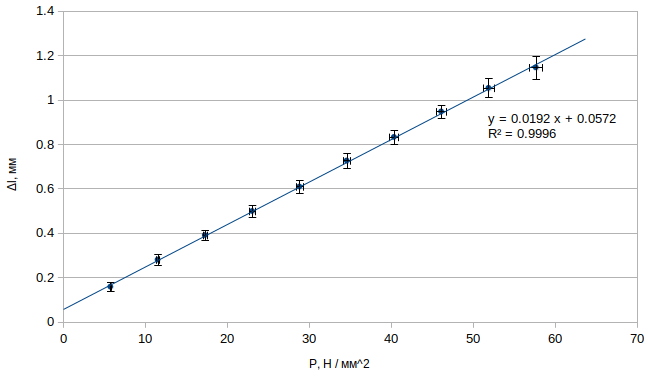
\includegraphics[scale=0.8]{131-132/graph1(2).png}
  \caption{График зависимости $\D{\ell}$ от P}
  \label{pic:2}
\end{figure}

Пусть a - наклон линии тренда, т.е. $\D{\ell} = aP$. Тогда
\[ a = (0.0192 \pm 0.0001) \frac{\H}{\mm^3} \]

$k = \frac{S}{a}$
\[ k = (21851 \pm 334) \H / \m \]

  \item \label{1:7} Найдем модуль Юнга проволки E и оценим погрешности.

$E = \frac{l_0}{a} = \frac{l_0 k}{S}$
\[ E = (91728 \pm 615) \H / \mm^2 \]
$\eps_a = 0.7\%,\ \eps_E = 0.7\%,\ \eps_k = 1.5\%$

{\center Смотрите таблицу (\ref{table:1})}

  \item \label{1:8}  Определим материал проволоки, сравнивая полученное значение с табличными.
  
Полученное значение попадает под:
\begin{enumerate} [label = \arabic*.]
  \item Латунь ($(78500 - 98100)\ \H / \mm^2$)
  \item Цинк ($(78500 - 98100)\ \H / \mm^2$)
\end{enumerate}

\end{enumerate}

\subsection{Вывод}
Целью первой части лабораторной работы было эксперементальное нахождение зависимости между напряжением и деформацией (закон Гука) для проволки и нахождение модуля Юнга проволки. Зависимость изображена на рисунке \refb{pic:2}, а полученные значения E и k можно посмотреть в таблице \refb{table:1}.

\section{Вторая часть.}

\paragraph{Цель работы}:
\begin{enumerate}
  \item определение модулей кручения и сдвига для проволоки по измерениям периодов крутильных колебаний подвешенного на ней маятника (динамический метод)
\end{enumerate}

\paragraph{Приборы}:
\begin{enumerate}
  \item проволока из исследуемого материала
  \item грузы
  \item секундомер
  \item микрометр
  \item линейка
\end{enumerate}

\subsection{Краткая Теория}

\begin{figure} [h] \center
  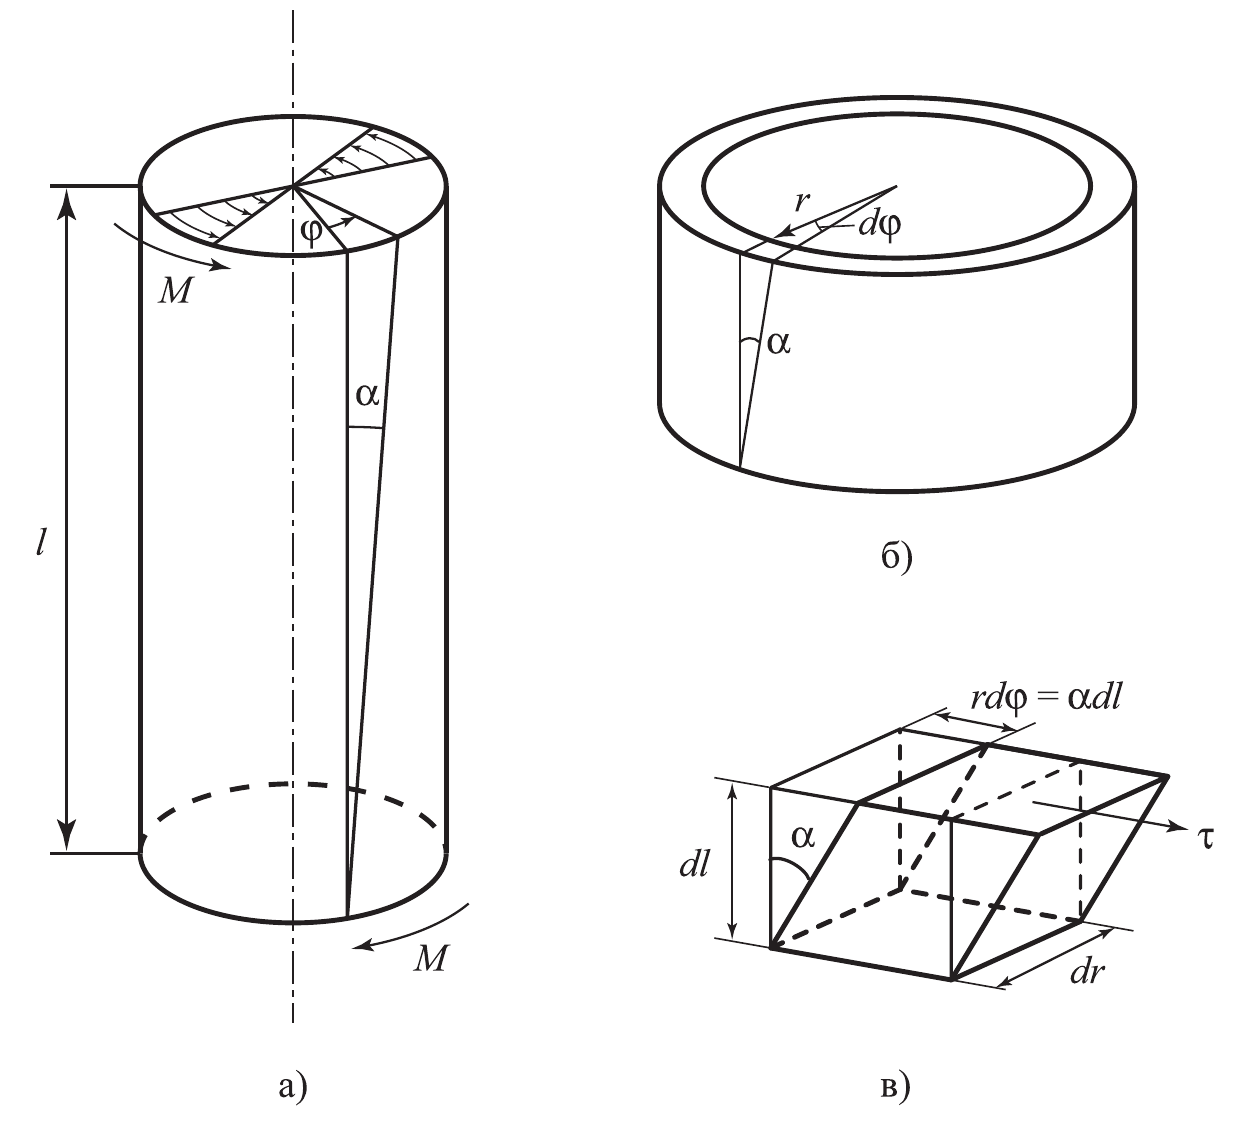
\includegraphics[scale = 0.5]{131-132/2 pic 1.png}
  \caption{Закручивание цилиндра. \label{pic:3}}
\end{figure}

Рассмотрим часть закручиваемого круглого цилиндра, имеющую длину $\ell$, которая изображена на рис. \ref{pic:3}. Любая прямаялиния,проведенная до закручивания цилиндра по частицам материала и параллельная оси симметрии, при закручивании превращается в спираль (винтовую линию). Сечения, находящиеся на расстоянии $\ell$, повернуты на угол $\varphi$.



\begin{equation}
  \alpha \d{\ell} = r \d{\varphi} {\label{eq:2.1}}
\end{equation}

\begin{equation}
  \tau = G \alpha \label{eq:2.2}
\end{equation}
, где $\tau$ - касательное напряжение, G - модуль сдвига.

\begin{equation}
  \tau = G r \deriv{\varphi}{l} \label{eq:2.3}
\end{equation}

\begin{equation}
  \d{M} = 2\pi r^2 \d{r} \tau \label{eq:2.4}
\end{equation}

\begin{equation}
  M = 2\pi G \deriv{\varphi}{l} \int_0^R{r^3 \d{r}} = 
  \pi G \deriv{\varphi}{l} \frac{R^4}{2} \label{eq:2.5}
\end{equation}

Этот момент не меняется по длине цилиндра.

\begin{equation}
  M = \frac {\pi G R^4}{2\ell} \varphi = f \varphi \label{eq:2.6}
\end{equation}

\begin{equation}
  f = \frac {\pi G R^4}{2\ell} \label{eq:2.7}
\end{equation}

M - момент сил на сечении.
Зависимость (\ref{eq:2.6}) выполняется при напряжениях намного меныших модуля сдвига, то есть при малых углах $\alpha$.

\begin{figure} [h] \center
  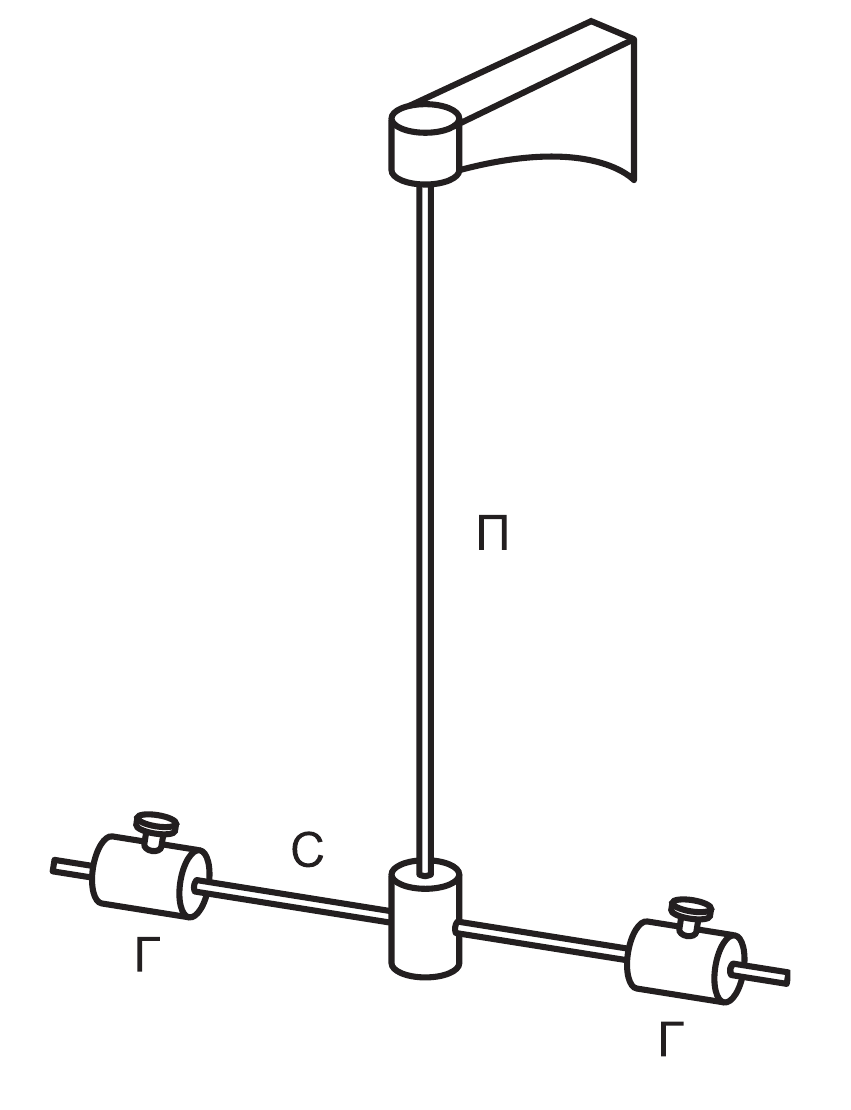
\includegraphics[scale = 0.5]{131-132/2 pic 2.png}
  \caption{Схема установки. \label{pic:4}}
\end{figure}

Экспериментальная установка, используемая во второй части работы,
изображена на рис. \ref{pic:4}. Она состоит из длинной вертикально висящей проволоки П, к нижнему концу которой прикреплен горизонтальный металлический стержень С с двумя симметрично расположенными грузами Г. Их положение на стержне можно менять и фиксировать.

При повороте на малый угол $\varphi$ будут возникать крутильные колебания.

\begin{equation}
  I \deriv[2]{\varphi}{t} = -M \label{eq:2.8}
\end{equation}
Здесь I — момент инерции стержня с грузами относительно оси вращения, $\varphi$ - угол поворота стержня от положения равновесия, М - момент сил.

\begin{equation}
  \w^2 = \frac{f}{I} \label{eq:2.9}
\end{equation}

\begin{equation}
  \deriv[2]{\varphi}{t} + \w^2\varphi = 0 \label{eq:2.10}
\end{equation}

\begin{equation}
  \varphi = \varphi_0 \sin{(\omega t + \theta)} \label{eq:2.11}
\end{equation}

\begin{equation}
  T = \frac{2\pi}{\omega} = 2\pi \sqrt{\frac{I}{f}} \label{eq:2.12}
\end{equation}

\subsection{Выполнение}
\begin{enumerate}
  \item[0] \label{2:0} Измерим длину проволки - L (см. таблицу \refb{table:5})
  \item \label{2:1} 
Прежде всего установим диапазон амплитуд, 
в котором применимы реультаты, полученные для незатухающих колебаний. Для этого закрепим грузы на некотором расстоянии от проволоки и возбудим в системе крутильные колебания. Измеряя время нескольких (не менее десяти) периодов колебаний, найдем период $T_1$. 
Уменьшив начальную амплитуду вдвое, тем же способом найдем соответствующий период $T_2$. Если $T_1 = T_2$, то для проведения измерений можно выбрать любую амплитуду не больше первой. Если окажется, что периоды не равны, то начальную амплитуду следует уменьшать до тех пор, пока не будетдостигнуто равенство этих периодов.

\centerline{Не выполняли.}

  \item \label{2:2} Убедимся в том, что после десяти периодов колебаний амплитуда уменьшается меньше, чем в два раза.

Убедились, но так как у нас не было необходимых приборов для измерения амплитуды, мы могли лишь примерно сказать, что амплитуда изменилась не сильно, пожтому данных, подтверждающих это, нет.
  
  \item \label{2:3} Установим грузы на стержне на одинаковом расстоянии $\ell$ от оси и измерим период колебаний Т. Проведем измерения для 4-6 различных значений $\ell$. (см. таблицу \refb{table:4}) Величину модуля кручения можно найти из наклона прямой, проведенной по экспериментальным точкам, отложенным в координатах $\ell^2,\ T^2$.
Построим график $T^2$ от $\ell^2$.
  
\begin{figure} [h] \center
  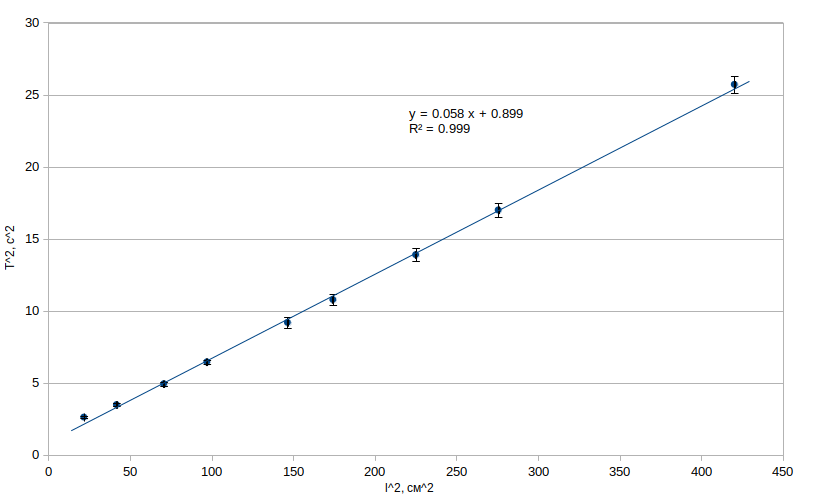
\includegraphics[scale = 0.6]{131-132/graph2(2).png}
  \caption{График зависимости $\ell^2, \cm^2$ от $T^2, \sec^2$. \label{pic:5}}
\end{figure}

\begin{table} [h] \center
\begin{tabular}{l|lllllllll}
&$\ell, \cm$&$\sigma_{\ell}$, см&$\eps_{\ell}$&N&$T_1$, с&$T_2$, с&T, с&$\sigma_{T}$, с&$\eps_T$\\
\hline
1&4.65&0.01&0.22\%&20&32.32&32.33&1.62&0.03&1.86\%\\
2&6.45&0.01&0.16\%&20&37.32&37.28&1.87&0.03&1.61\%\\
3&8.40&0.01&0.12\%&20&44.38&44.38&2.22&0.03&1.35\%\\
4&9.85&0.01&0.10\%&20&50.79&50.79&2.54&0.03&1.18\%\\
5&12.10&0.01&0.08\%&10&30.31&30.3&3.03&0.06&1.98\%\\
6&13.20&0.01&0.08\%&10&32.84&32.8&3.28&0.06&1.83\%\\
7&15.00&0.01&0.07\%&10&37.28&37.25&3.73&0.06&1.61\%\\
8&16.60&0.01&0.06\%&10&41.22&41.22&4.12&0.06&1.46\%\\
9&20.50&0.01&0.05\%&10&50.7&50.7&5.07&0.06&1.18\%\\
\end{tabular}
\caption{Измерения \label{table:4}}
\begin{description}
  \item[$\ell$] - рассояние от оси вращения системы до центров масс грузов
  \item[N] - кол-во колебаний
  \item[$T_i$] - измеренное время
  \item[T] - период колебаний
\end{description}
\end{table}

\begin{table} [h] \center
\begin{tabular}{l|llllll}
&$\ell^2,\ \cm^2$&$\sigma_{\ell^2}, \cm^2$&$\eps_{\ell^2}$&$T^2, \sec^2$&$\sigma_{T^2}, \sec^2$&$\eps_{T^2}$\\
\hline
1&21.6&0.1&0.4\%&2.6&0.1&4\%\\
2&41.6&0.1&0.3\%&3.5&0.1&3\%\\
3&70.6&0.2&0.2\%&4.9&0.1&3\%\\
4&97.0&0.2&0.2\%&6.4&0.2&2\%\\
5&146.4&0.2&0.2\%&9.2&0.4&4\%\\
6&174.2&0.3&0.2\%&10.8&0.4&4\%\\
7&225.0&0.3&0.1\%&13.9&0.5&3\%\\
8&275.6&0.3&0.1\%&17.0&0.5&3\%\\
9&420.3&0.4&0.1\%&25.7&0.6&2\%\\
\end{tabular}
\caption{Значения для графика на рис. \refb{pic:5}}
\end{table}


Пусть a - наклон линии тренда, т.е. $T^2 = a \ell^2 + b$. Тогда
\[ a = (0.058 \pm 0.001) \frac{\sec^2}{\cm^2} \]
$\eps_a = 1.12\%$
{
\[ \eqref{eq:2.12} \implies 
T^2 = \frac{4\pi^2 I}{f} = 
\frac{4\pi^2}{f} (I_\text{гр} + I_0) =
\frac{4\pi^2 (m_1+ m_2)}{f} \ell^2 + \frac{4\pi^2 I_0}{f}\]

Здесь I - общий момент инерции системы (см. рис. \refb{pic:4}), 
$I_\text{гр}$ - момент инерции двух грузов, 
$I_0$ - момент инерции установки, 
$m_1, m_2$ - массы грузов.

\[a = \frac{4\pi^2 (m_1 + m_2)}{f} \implies f = \frac{4\pi^2 (m_1 + m_2)}{a} \]

\[\sigma_f = f \cdot \sqrt{\eps_m^2 + \eps_a^2}\]
}

\[ f = (27.5 \pm	0.3)\ \H \cdot \mm \]
$\eps_f = 1.12\%$

  \item \label{2:4}  Измерим диаметр проволоки П (см. таблицу \ref{table:5}). По найденному модулю кручения с помощью формулы \eqref{eq:2.7} получим модуль сдвига G, оценим погрешность и сравним с табличными значениями в справочниках.
  
$\eqref{eq:2.7} \implies G = \frac{2 l f}{\pi R^4}$
  
\[ G =  (43 \pm 1)\ \gPa \]
$\eps_G = 1.3\%$

Значение G попадает в табличное значение для меди и не только, но, скорее всего, это наша проволка сделана из меди.

\begin{table} [h] \center
\begin{tabular}{l|lll}
&значение&$\sigma$&$\eps$\\
\hline
$m_1$, г&202.5&0.1&0.05\%\\
$m_2$, г&204.1&0.1&0.05\%\\
m, г&203.3&0.1&0.05\%\\
h&4&0.01&0.3\%\\
a, $\sec^2/\cm^2$&0.058&0.001&1.12\%\\
$\fint$, Н*мм&27.5&0.3&1.12\%\\
G, $\gPa$&43&1&1.30\%\\
L, см&100&0.01&0.01\%\\
D, мм&1.5052&0.005&0.3\%\\
R, мм&0.7526&0.0025&0.3\%\\
время&&0.6&\\
\end{tabular}
\caption{Значения \label{table:5}}
\begin{description}
  \item[$m_1$ и $m_2$] - массы грузов
  \item[m] - ср. знач. $m_1$ и $m_2$ 
  \item[h] - ширина грузов (расстояние от края до центра масс)
  \item[a] - наклон прямой на рис. \refb{pic:5} 
  \item[f] - модуль кручения проволки
  \item[G] - модуль сдвига проволки
  \item[L] - длина проволки П установки
  \item[D и R] - диаметр и радиус проволки П
\end{description}
\end{table}

\begin{table} [h] \center
\begin{tabular}{l|l}
&d, мм\\
\hline
1&1.505\\
2&1.505\\
3&1.505\\
4&1.505\\
5&1.505\\
6&1.506\\
7&1.505\\
8&1.506\\
9&1.505\\
10&1.505\\
\end{tabular}
\caption{Измерения диаметра проволки. \label{table:6}}
\end{table}

\end{enumerate}

\subsection{Вывод}
Во второй части лабораторной работы мы определили модули кручения и сдвига для проволоки по измерениям периодов крутильных
колебаний подвешенного на ней маятника. Поняли из какого материала сделана наша проволка.

\end{document}